\chapter{Testing and Verification}
Testing and verification are used to verify the correctness of the DLX. Testing can be defined as the process of observing and verifying the results of a component under specific conditions in order to find possible inconsistencies between the actual and the required behaviour.

The flow used to verify a component follows multiple steps:
\begin{itemize}
	\itemsep0sp
	\item Creation of the Testbench
	\item Simulation
	\item Post Synthesis simulation (after the Synthesis and Optimization, refer to section \ref{sec:syn_opt})
\end{itemize}

\section{Testbenches}
All Testbenches developed for the DLX verification have been implemented using VHDL. The most critical components have been tested with their own testbenches, like:
\begin{itemize}
	\itemsep0sp
	\item Booth's multiplier
	\item P4 adder
	\item Comparator
	\item ALU
	\item Shifter
	\item Windowing Register File
\end{itemize}
The smaller components have been intensively tested while verifying the correct behaviour of the DLX itself.\newline\newline

The DLX Testbench is implicitly based on two processes; the first one manages and creates only the clock signal with a period of 1 ns, while the second one asserts the reset signal for the first clock period and then negates it in order to start the correct test execution.

To create the most flexible test possible multiple components have been instantiated; these provide all the external interfaces the DLX needs. So, besides the DLX instance, the Testbench also contains the following component:
\begin{itemize} 
	\item Instruction RAM (IRAM): this is a read only memory that takes an external file, in this case a .mem file, and uses it as a source for fetching the instruction. When the reset is performed, all the instructions in the file are written in an internal array of 32 bits. At each clock cycle, the array is indexed with an index that comes from outside, that corresponds to the DLX \texttt{PC}.
	\item Data RAM (DRAM): similarly to the IRAM, the DRAM is loaded at the startup using the same .mem explained before. In fact, this compiled file does not only contain the code instructions but, after a blank line, also the memory content the program should have once it starts. Since a DRAM must also be writable, the memory is implemented as a read/write one. 
	
	To simplify the verification of the memory content, each time a value is written the external file, that is the exact copy of the DRAM content, is updated too.
	In order to correctly access the data that are stored in the memory, the address comes from outside and corresponds to the one used in the Memory Stage (refer to \ref{chp:memory_stage}).
	
	To replicate a more realistic environment and increase the test reliability, the DRAM has been enhanced with a \texttt{ready} signal that is `1' when it is ready. This has been implemented with a counter, that only after \texttt{data\_delay} clock cycles makes the memory ready and allows to generate a meaningful value.
	
	Last but not least, the DRAM must be able to correctly manage all the different data sizes, both during the write and the read operation. So, an additional signal on two bits, called \texttt{MAS}, has been included. A more accurate description of the memory data size management is available in section \ref{mas}.
\end{itemize}

The reduction of the setup time needed to starting a new simulation was a crucial point to speed up the entire verification process. For this reason, a bash script has been develop in order to generate the .mem file from an .asm one a move it into the correct testing folder. This allows to need only to change the the .mem file reference in the Testbench. The bash script is the one at Appendix \ref{code:asm_script}.



\section{Simulation}
The verification of the behaviour of the DLX is based on the simulation of the DLX itself, using the Testbench wrote in the previous phase. Before starting the simulation, all the components must be compiled; an organizational improvement has been added for simplifying the compilation file organization. The folder structure is based on a hierarchical organization of the components, by using the alphabet letters as starting name. Each folder includes a \texttt{compile.script} file that is used to compile all the files in the folder and call all the others \texttt{compile.script} files in the sub-folders. Folders are organized in the following way:

\hfill

\dirtree{%
	.1 DLX\_vhd\_fully\_synthesizable/.
	.2 compile.script.
	.2 a.b-DataPath.core/.
	.3 compile.script.
	.3 a.b.a-windowedRF.core/.
	.4 compile.script.
	.3 a.b.d-ALU.core/.
	.4 compile.script.
	.4 a.b.d.c-adder.core/.
	.5 compile.script.
	.4 a.b.d.b-multiplier.core/.
	.5 compile.script.
	.2 a.d-decode.core/.
	.3 compile.script.
	.2 test\_bench\_and\_memory/.
	.3 compile.script.
	.3 TB\_packages/.
	.4 compile.script.
	.3 TB\_romem/.
	.4 compile.script.
	.3 TB\_rwmem/.
	.4 compile.script.
}

\hfill


Once \textit{Questa Sim} is loaded, the \texttt{DLX\_vhd\_fully\_synthesizable/compile.script} can be executed using the \texttt{source} command. After a while, all the components of the DLX will be compiled. Another TCL script, called \texttt{launch\_sim\_waves.script} (refer to Appendix \ref{sim_wave}), has been developed in order to start the simulation and load the waves of the registers from \texttt{R0} to \texttt{R31} in the Wave view.

\begin{figure}[H]   
	\centering
	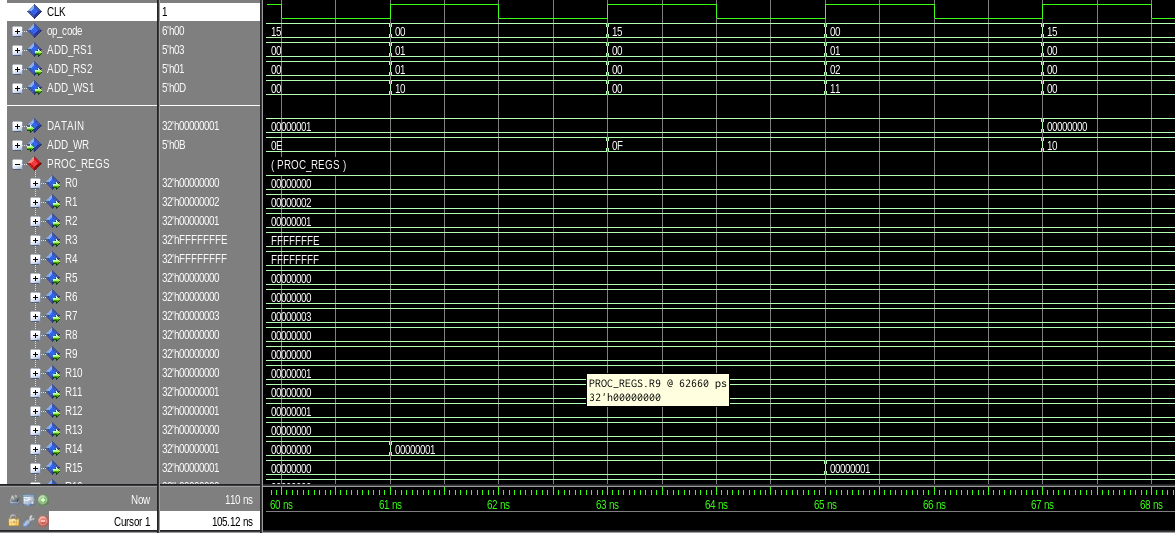
\includegraphics[width=0.85\textwidth]{chapters/8_TestingVerification/images/simulation.png}
	\caption{Questa Sim Simulation}
	\label{fig:simulation}
\end{figure}

\section{Post Synthesis Simulation}
After the Synthesis and Optimization phase, which allows to improve the circuit under multiple points of view and perform the tech mapping, it's possible to simulate the behaviour of the circuit using the standard cells.

Another script, that is similar to the \texttt{launch\_sim\_waves.script} one has been created in order to manage the standard cells. Basically, the script used for the synthesized circuit, called \texttt{launch\_sim\_synthesis.script}, instead of simply starting the simulation also needs to link the \textit{nangate45} library. It can be done by using the following line:
\begin{lstlisting}
	vsim work.dlx_testbench -t ns -L /software/dk/nangate45/verilog/qsim10.7c 
\end{lstlisting}
